\documentclass{beamer}



%\usepackage{beamerthemesplit}
\usetheme{Boadilla}
%\usetheme{default}
%\useinnertheme{rounded}

%\useoutertheme{shadow}
\usecolortheme{rose}
%\usefonttheme{serif}
\setbeamertemplate{navigation symbols}{}
\usetheme{Madrid}

\usepackage{amssymb,amsmath,amscd,amsfonts,amsthm,dsfont,color,graphicx}
\usepackage{amscd}
%\usepackage[numbers]{natbib}
% \usepackage[french]{babel}
%\usepackage[active]{srcltx}


% \date[]{}

 \newcommand\makebeamertitle{\frame{\maketitle}}%

 \AtBeginDocument{
   \let\origtableofcontents=\tableofcontents
   \def\tableofcontents{\@ifnextchar[{\origtableofcontents}{\gobbletableofcontents}}
   \def\gobbletableofcontents#1{\origtableofcontents}
 }
\numberwithin{equation}{section}
  \theoremstyle{plain}
  \newtheorem*{thm*}{\protect\theoremname}
  \theoremstyle{plain}
  \newtheorem*{cor*}{\protect\corollaryname}
 \theoremstyle{definition}
 \newtheorem*{defn*}{\protect\definitionname}
 \theoremstyle{plain}
\newtheorem*{lem*}{\protect\lemmaname}
  \theoremstyle{plain}
  \newtheorem*{rem*}{\protect\remarkname}
   \theoremstyle{definition}
 \newtheorem*{prop*}{\protect\propositionname}

\usetheme{Madrid}

\makeatother

  \providecommand{\corollaryname}{Corollary}
  \providecommand{\definitionname}{Definitioninition}
  \providecommand{\theoremname}{Theorem}
   \providecommand{\lemmaname}{Lemma}
   \providecommand{\remarkname}{Remark}
   \providecommand{\propositionname}{Proposition}
   
   


\newcommand{\Rl}{\mathbb{R}}
\newcommand{\Cplx}{\mathbb{C}}
\newcommand{\Itgr}{\mathbb{Z}}
\newcommand{\Ntrl}{\mathbb{N}}
\newcommand{\Circ}{\mathbb{T}}
\newcommand{\Sb}{\mathbb{S}}
\newcommand{\Disc}{\mathbb{D}}
\newcommand{\Aff}{\mathbb{A}}

% The Caligraphic alphabet
\newcommand{\Ac}{\mathcal{A}}
\newcommand{\Bc}{\mathcal{B}}
\newcommand{\Cc}{\mathcal{C}}
\newcommand{\Dc}{\mathcal{D}}
\newcommand{\Ec}{\mathcal{E}}
\newcommand{\Fc}{\mathcal{F}}
\newcommand{\Gc}{\mathcal{G}}
\newcommand{\Hc}{\mathcal{H}}
\newcommand{\Ic}{\mathcal{I}}
\newcommand{\Jc}{\mathcal{J}}
\newcommand{\Kc}{\mathcal{K}}
\newcommand{\Lc}{\mathcal{L}}
\newcommand{\Mv}{\mathcal{M}}
\newcommand{\Nv}{\mathcal{N}}
\newcommand{\Oc}{\mathcal{O}}
\newcommand{\Pc}{\mathcal{P}}
\newcommand{\Qc}{\mathcal{Q}}
\newcommand{\Rc}{\mathcal{R}}
\newcommand{\Sc}{\mathcal{S}}
\newcommand{\Tc}{\mathcal{T}}
\newcommand{\Uc}{\mathcal{U}}
\newcommand{\Vc}{\mathcal{V}}
\newcommand{\Wc}{\mathcal{W}}
\newcommand{\Xc}{\mathcal{X}}
\newcommand{\Yc}{\mathcal{Y}}
\newcommand{\Zc}{\mathcal{Z}}


\newcommand{\Sp}{\mathrm{Sp}}
\newcommand{\tr}{\mathrm{tr}}
\newcommand{\Op}{\mathrm{Op}}
\newcommand{\sym}{\mathrm{sym}}
\newcommand{\Vol}{\mathrm{Vol}}
\newcommand{\Tr}{\mathrm{Tr}}
\newcommand{\dist}{\mathrm{dist}}
\newcommand{\sgn}{\operatorname{sgn}}
\newcommand{\diag}{\mathrm{diag}}
\newcommand{\id}{\mathrm{id}}
\newcommand{\Poly}{\mathrm{Poly}}

\newcommand{\spec}{\mathrm{Spec}}
\newcommand{\abs}{\mathrm{abs}}

\newcommand{\CV}{\mathrm{CV}}
\newcommand{\PCV}{\mathrm{PCV}}


% Used for highlighting. To remove all highlighting just make the command blank
\newcommand{\hl}{\color{red}}


\newcommand{\gf}{\mathfrak{g}}
\newcommand{\tf}{\mathfrak{t}}
\newcommand{\Str}{\mathrm{STr}}



\newcommand{\dom}{\mathrm{dom}}
\newcommand{\supp}{\mathrm{supp}}
\newcommand{\BS}{\mathfrak{BS}}
\newcommand{\loc}{\mathrm{loc}}
\newcommand{\re}{\mathrm{re}}
\newcommand{\im}{\mathrm{im}}

% DOI transformer
\newcommand{\Ti}{\mathcal{T}}


\DeclareMathOperator{\Ext}{\mathsf{\Lambda}}


\def\Xint#1{\mathchoice
{\XXint\displaystyle\textstyle{#1}}%
{\XXint\textstyle\scriptstyle{#1}}%
{\XXint\scriptstyle\scriptscriptstyle{#1}}%
{\XXint\scriptscriptstyle\scriptscriptstyle{#1}}%
\!\int}
\def\XXint#1#2#3{{\setbox0=\hbox{$#1{#2#3}{\int}$ }
\vcenter{\hbox{$#2#3$ }}\kern-.6\wd0}}
\def\qint{\Xint-}

\def\qd{\,{\mathchar'26\mkern-12mu d}}

\newcommand{\CR}{\mathrm{CR}}
   
   
   
\begin{document}

\title[Introduction to the Hypoelliptic Laplacian]{Introduction to the Hypoelliptic Laplacian on a compact group}


\author[E. McDonald]{Ed McDonald\\
Based on joint work with N.~Higson, S.~Liu, F.~Sukochev and D.~Zanin}


\institute[]{Penn State University}

\makebeamertitle

\begin{frame}{Introduction}
  The \textbf{hypoelliptic Laplacian} of J.~M.~Bismut has an intimidating reputation.
  
  \pause
  But... where does it come from?\\
  \pause
  What is it good for?\\
  \pause
  And, most importantly, how do we prove things about it?
\end{frame}

\section{Frenkel's formula}

\begin{frame}
  \huge{Section 1: Frenkel's formula}
\end{frame}

\begin{frame}
  Let $G$ be a connected, simply connected, compact group, with Lie algebra $\gf$ having nondegenerate bilinear form $B.$
  
  Specify a Cartan subalgebra $\tf \subset \gf$ and corresponding maximal abelian subgroup $T\subset G.$
  We have the co-root lattice
  \[
    \CR = \{X \in \tf\;:\; \exp(X) = 1_G\}
  \]
  and the weight lattice 
  \[
  \CR^* = \{\lambda \in \tf^*\;:\; \lambda(X) \in \Itgr,\quad X \in \CR\}
  \]
  with specified positive subspace $\CR_+^*\subset \CR^*.$
  
  There is the Casimir element, $\Delta_G \in \Uc(\gf).$
   
  What is $\Tr(e^{t\Delta_G})$? 
\end{frame}

\begin{frame}{What is $\Tr(e^{t\Delta_G})$}
  Some possible answers:
  \begin{enumerate}
    \item{} Spectral (Peter-Weyl) representation: we have
    \[
        \Tr(e^{t\Delta_G}) = \sum_{\lambda\in CR^*_+} \left(\prod_{\alpha>0} \frac{B(\alpha,\rho+\lambda)}{B(\alpha,\rho)}\right)^2e^{-tB(\lambda+2\rho,\lambda)}
    \]
    where $\prod_{\alpha>0}$ is the product over positive roots, $\rho$ is the Weyl element.
    \item{} Minakshisundaram-Pleijel expansion: asymptotically, as $t\to 0,$ we have
    \[
        \Tr(e^{t\Delta_G}) \sim (4\pi t)^{-\frac{\mathrm{dim}(G)}{2}}(a_0+a_1t+a_2t^2+\cdots)
    \]
    where 
    \[
      a_n = \frac{\mathrm{Vol(G)}}{n!}(2\pi B(\rho,\rho))^{2n}.
    \]
  \end{enumerate}
  \pause
  Is there a ``better" representation?
\end{frame}

\begin{frame}{Jacobi identity}
  If $G = \Circ$ is the unit circle, the answer is \emph{yes}. We have
  \[
    \Tr(e^{t\Delta_{\Circ}}) = \frac{\mathrm{Vol}(\Circ)}{(4\pi t)^{\frac12}}\sum_{n\in \Itgr} e^{-\frac{1}{4t}n^2}.
  \]
  We can prove this via the Poisson summation formula and the fact that
  \[
    \Tr(e^{t\Delta_{\Circ}}) = \sum_{n\in \Itgr} e^{-tn^2}
  \]
  
  Is there something similar for a general Lie group?
\end{frame}

\begin{frame}{Frenkel's formula}
  It turns out that we get a cleaner statement by considering a ``shifted" version
  \[
    \Tr(\lambda(e^H)e^{t\Delta_G})
  \]
  where $H\in \tf,$ and $\lambda(e^H)$ is the left shift operator by $e^H\in G.$
  \begin{theorem}[\`{E}skin (1964), Frenkel (1984)]
      If $H\in \tf$ is regular (i.e., $\alpha(H)\neq 0$ for all roots $\alpha$), then
      \begin{align*}
          &\Tr(\lambda(e^H)e^{t\Delta_G})\\
          &= \frac{\mathrm{Vol}(G)e^{4\pi^2tB(\rho,\rho)^2}}{(4\pi t)^{\frac{\mathrm{dim}(G)}{2}}\sigma(H)}\sum_{\gamma \in CR} \left(\prod_{\alpha>0} \langle \alpha,H+\gamma\rangle\right) e^{-\frac{1}{4t}B(H+\gamma,H+\gamma)}
      \end{align*}
      where $\sigma$ is the Weyl denominator.
  \end{theorem}
  \pause
  We can also take $H\to 0,$ but the resulting expression for $\Tr(e^{t\Delta_G})$ is more complicated, see \`{E}skin's paper.
\end{frame}

\begin{frame}{Proof of Frenkel's formula}
    Frenkel proved his formula using the explicit spectral decomposition of $\Delta_G$ and the Weyl character formula. From these facts, we have
    \begin{align*}
      &\Tr(\lambda(e^H)\rho(e^K)e^{t\Delta_G})\\ 
      &= \sum_{\lambda \in CR^*_+} \frac{1}{\sigma(H)\sigma(K)}\left(\sum_{w \in W} \sgn(w)e^{w(\lambda+\rho)(H)}\right)\\
      &\quad \cdot \left(\sum_{w\in W} \sgn(w)e^{w(\lambda+\rho)(K)}\right)e^{-tB(\lambda+2\rho,\lambda)}
    \end{align*}
    (here, $\rho$ is the right-regular representation).
    Some rearrangement, Poisson's summation formula, and sending $K\to 0$ gives the result.
\end{frame}

\begin{frame}{Remarks on Frenkel's formula}
If we examine Frenkel's formula
\begin{align*}
 &\sum_{\lambda \in CR^*_+} \frac{1}{\sigma(H)\sigma(K)}\left(\sum_{w \in W} \sgn(w)e^{w(\lambda+\rho)(H)}\right)\\
      &\quad \cdot \left(\sum_{w\in W} \sgn(w)e^{w(\lambda+\rho)(K)}\right)e^{-tB(\lambda+2\rho,\lambda)}\\
      &=\frac{\mathrm{Vol}(G)e^{4\pi^2tB(\rho,\rho)^2}}{(4\pi t)^{\frac{\mathrm{dim}(G)}{2}}\sigma(H)}\sum_{\gamma \in CR} \left(\prod_{\alpha>0} \langle \alpha,H+\gamma\rangle\right) e^{-\frac{1}{4t}B(H+\gamma,H+\gamma)}
\end{align*}
We can see that a sum over the \emph{weight lattice} is converted into a sum over the \emph{coroot lattice}. The exponential $\exp(-tx^2)$ is converted to $\exp(-\frac{1}{t}x^2).$ (as if this were a Fourier transform).
\end{frame}

\begin{frame}{Looking to Bismut}
Bismut gave a new proof of Frenkel's formula, which is really a lot more complicated than Frenkel's proof. But it differs in some essential ways:
\begin{itemize}
  \item{} Bismut does not use the Peter-Weyl decomposition of $G.$ The proof involves very little information from the representation theory of $G.$
  \item{} The coroot lattice $\CR$ of $G$ emerges in a purely geometric way, rather than as the dual of the weight lattice.
\end{itemize}
\end{frame}

\begin{frame}
    \huge{Section 2: The Primordial History, or, the Duistermaat--Heckman localisation formula}
\end{frame}

\begin{frame}{In the beginning...}
  In this section, I will attempt to give a ``folkloric" story for the origins of the hypoelliptic Laplacian.
  
  I am strongly indebtted to the paper of Choi--Takhtajan (2021) for this explanation.
\end{frame}

\begin{frame}{The Hamiltonian-Lagrangian correspondence}
  In its most general terms, the path integral method in quantum mechanics relates traces of semigroups
  to integrals over loop space. 
  
  The way it is supposed to work is as follows: $X$ is a manifold, and $\Lc \in C^\infty(TX)$ is a ``Lagrangian". The corresponding
  ``Hamiltonian" $\Hc\in C^\infty(T^*X)$ is related to $\Lc$ by the Legendre transform 
  \[
    \Hc(x,p) = \sup_{X \in T_xX} (p(X)-\Lc(x,X)),\quad (x,p) \in T^*X.
  \]
\end{frame}

\begin{frame}{The Hamiltonian-Lagrangian correspondence}
  We are supposed to have something like the following:
  \begin{equation}
    \Tr(e^{-t\Hc(x,-i\partial)}) = \int_{L_tX} e^{-\int_0^t \Lc(\gamma(s),\dot{\gamma}(s))\,ds} \Dc \gamma.
  \end{equation}
  Here, $\Hc(x,-i\partial)$ is an operator on the Hilbert space $L_2(X)$ defined by some kind of quantisation of $\Hc,$ $L_tX$ is the space of loops of ``time" $t,$ that is functions $\Rl/t\Itgr \to X,$ and ``$\Dc\gamma$" is some kind of measure on loop space.\\
  
  \pause
  Both sides of this formula are problematic, but the left-hand-side is a bit more accessible. 
\end{frame}

\begin{frame}{The Hamiltonian-Lagrangian correspondence}
  One case (and one of the few cases that is well-understood) is for $\Delta_g,$ the Laplace operator on a compact Riemannian manifold
  \[
    \frac12\Delta_gu = \frac12\det(g)^{-\frac12}\partial_{\alpha}(g^{\alpha,\beta}\det(g)^{\frac12}\partial_{\beta}u)
  \]
  This is supposed to be $\Hc(x,-i\partial),$ where $\Hc(x,p) = \frac12 g^{\alpha,\beta}(x)p_{\alpha}p_{\beta}.$ The corresponding Lagrangian is
  \[
    \Lc(x,X) = \frac12 g_{\alpha,\beta}(x)X^{\alpha}X^{\beta}
  \]
  and
  \[
    \Tr(e^{\frac12 t\Delta_g}) = \int_{L_tX} e^{-\frac{1}{2}\int_0^t g_{\alpha,\beta}(\gamma(s))\dot{\gamma}^{\alpha}(s)\dot{\gamma}^\beta(s)\,ds}\, \Dc \gamma
  \]
  where the integral on the right-hand side can be rigorously defined as a limit of discrete approximations. See Andersson--Driver (1998).
\end{frame}

\begin{frame}{Duistermaat--Heckman formula}
  Let $(X,\omega)$ be a symplectic $n$-manifold. The symplectic volume form of $X$ is $\frac{1}{(n/2)!}\omega^{\frac{n}{2}} = \exp(\omega).$

  Let $H\in C^\infty(X),$ and suppose that $H$ has isolated and non-degenerate critical points. Laplace's asymptotic formula tells us that as $t\to\infty,$ we have
  \[
    \int_{X} \exp(-tH) \frac{\omega^{n/2}}{(n/2)!} \sim \sum_{p} \frac{\exp(-tH(p))}{t^{n/2}\det^{\frac12}(2\pi \nabla^2 H(p))}
  \]
  Here the sum is over the critical points of $H.$
\end{frame}

\begin{frame}{Duistermaat--Heckman formula}
  $(X,\omega)$ is a symplectic $n$-manifold.
  \begin{theorem}
      Suppose that there is a circle action $\Circ\times X\to X$ with isolated fixed points, and let its derivative be the vector field $V.$ If $V$ is Hamiltonian, with Hamiltonian function $H,$ then
      \[
          \int_X \exp(-tH) \frac{\omega^{n/2}}{(n/2)!} = \sum_{p} \frac{\exp(-tH(p))}{t^{n/2}\det^{\frac12}(2\pi \nabla^2 H(p))}
      \]
  \end{theorem}
  \pause
  That is to say, for Hamiltonians coming from a circle action, the Laplace asymptotic expansion is exact.
\end{frame}

\begin{frame}{Proof of Duistermaat--Heckman localisation}
    Duistermaat-Heckman can be proved by introducing a new parameter $b$ in the following way: It is possible to construct a differential form $\Vc \in \Omega^{\bullet}(X)$ such that
    \[
      \int_X \exp(-tH+\omega) = \int_Z \exp(-tH+\omega+b\Vc)\quad b>0.
    \]
    This is proved by showing that the right hand side is independent of $b,$ and then setting $b=0.$ The limit as $b\to\infty$ is computed using Laplace's asymptotic formula.
\end{frame}

\begin{frame}{Bismut's dream}
  We would like to compute $\Tr(e^{t\Delta_g})$ by considering
  \[
    \int_{L_tX} e^{-\int_0^t \frac12 g_{\alpha,\beta}(\gamma(s))\dot{\gamma}^{\alpha}(s)\dot{\gamma}^\beta(s)\,ds} \Dc\gamma
  \]
  as an integral of a differential form over the infinite dimensional manifold $LX.$
  Note that $LX$ has a $\Circ$-action given by rotating around the loop.
  \\
  There are reasons to think that this should be a Hamiltonian action, with Hamiltonian function
  \[
  \int_0^1 \frac12 g_{\alpha,\beta}(\gamma(s))\dot{\gamma}^{\alpha}(s)\dot{\gamma}^\beta(s)\,ds
  \]
  \pause
  This theme was very popular in the 1980s -- it led ultimately to Getzler's proof of the local index formula.  
  \pause
  We could try to mimic the proof of Duistermaat--Heckman by introducing a $1$-parameter perturbation of $\Lc,$ something like
  \[
      \int_{LX} e^{-\int_0^t \Lc(\gamma(s),\dot{\gamma}(s))+b\Vc\,ds} \Dc\gamma
  \]
  where $b>0,$ and computing the limit as $b\to\infty.$
  \pause
  This is \textbf{TOO HARD}.
\end{frame}

\begin{frame}{Bismut's dream}
  Doing Duistermaat--Heckman in loop space is a great idea but it's too difficult to attempt directly.
  
  But maybe, we can use the Hamiltonian-Lagrangian correspondence to replace incomprehensible loop space integrals with slightly more comprehensible operator traces.
  \begin{center}
    Can we find an operator $\Lc_b$ depending on a parameter $b$ such that
    \[
      \Tr(e^{t\Delta_g}) = \Tr(e^{t\Lc_b})
    \]
    for all $b>0,$ and such that the limit as $b\to\infty$ expresses the trace as a sum over geodesics?
  \end{center}
  \textbf{Answer}: In a way, yes. Not precisely as stated above, but we can get close enough.
\end{frame}

\begin{frame}{The hypoelliptic Laplacian}
  Let $G$ be a compact Lie group, we consider $\Delta_G$ rather than the general $\Delta_g.$ Through some combination of path integral computations, intuition, and guesswork, Bismut found a solution the preceding question.
  \begin{theorem}[Bismut (2011)]
    Let $H\in \tf$ be regular. There is a differential operator $\Lc_{b},$ depending on a positive real parameter $b,$ acting on the space
    \[
      C^\infty(\gf\times G,\Ext^\bullet\gf)
    \]
    such that for $H \in \tf$ we have
    \[
       \Tr(\lambda(e^H)e^{t(\Delta_G+C)}) = \Str(\lambda(e^H)e^{-t\Lc_{b}}),\quad b>0.
    \]
    where $C$ is a scalar.
    As $b\to\infty,$ it can be proved that $\Str(\lambda(e^H)e^{-t\Lc_{b}})$ converges to Frenkel's formula.
  \end{theorem}
\end{frame}

\section{The form of $\Lc_b.$}

\begin{frame}
  \huge{Section 3: The form of $\Lc_b$}
\end{frame}

\begin{frame}{Notation}
  $G$ is a compact Lie group of dimension $d,$ and $\gf$ is its Lie algebra with positive-definite bilinear form $B$. Let $e_1,\ldots,e_d$ be an orthonormal basis of $\gf.$
  
  We will write the variables of $\gf\times G$ as $(y,x),$ and we have Clifford operators on $\Ext^{\bullet}\gf,$ denoted
  \[
    c(v) = v\wedge + \iota_v,\quad \widehat{c}(v) = v\wedge -\iota_v,\quad v \in \gf.
  \]
  These satisfy the Clifford relations
  \[
    c(v)c(w)+c(w)c(v) = 2B(v,w),\quad \widehat{c}(v)\widehat{c}(w)+\widehat{c}(w)\widehat{c}(v) = -2B(v,w).
  \]
\end{frame}

\begin{frame}{Definition of $\Lc_b.$}
  It would be nice to have a heuristic derivation of $\Lc_b$ that follows from the path integral computations, but I am not convinced that such a thing exists. Instead, let's take Bismut at his word and assert the following definition.
  \begin{definition}
    \[
      \Lc_b = (D+\frac1bQ)^2-D^2
    \]
  \end{definition}
  where
  \[
    Q = \sum_{j=1}^d c(e_j)y_j-i\widehat{c}(e_j)\partial_{y_j}
  \]
  and 
  \[
    D = \sum_{j=1}^d -ic(e_j)\partial_{x_j}+\frac{1}{12}f^j_{k,l}c(e_j)c(e_k)c(e_\ell)
  \]
  is the \emph{Kostant Dirac operator} on $G.$ Note that $D^2  =-\Delta_G+C.$
\end{frame}

\begin{frame}{Structure of $\Lc_b.$}
  Expanding out the definitions, we get
  \[
    \Lc_b = \frac{1}{b^2}Q^2+\frac{1}{b}(QD+DQ)
  \]
  which turns out to be
  \[
    \Lc_b = \frac{1}{b^2}\sum_{j=1}^d y_j^2-\partial_{y_j}^2 + \frac{1}{b}\sum_{j=1}^dy_j\partial_{x_j} + \text{matrix terms.}
  \]
  \pause
  This operator satisfies H\"ormander's condition, and is therefore hypoelliptic.
\end{frame}


\section{Section 4: the world's most convoluted proof of Frenkel's formula}

\begin{frame}
  \huge{Section 4: The world's most convoluted proof of Frenkel's formula}
\end{frame}

\begin{frame}{The main tasks}
  Ultimately, we want to show the following facts:
  \begin{itemize}
    \item{} $\lim_{b\to 0} e^{-t\Lc_b} = e^{-tD^2}$ \emph{in the correct sense},
    \item{} $\lim_{b\to \infty} \Str(\lambda(e^H)e^{-t\Lc_b}) = \text{Frenkel's formula.}$
  \end{itemize}
  \pause
  Of course, to state these questions we need to determine if $\exp(-t\Lc_b)$ even exists and belongs to the trace class.
\end{frame}


\begin{frame}{The limit as $b\to 0.$}
    In some sense, we are supposed to have
    \[
      \exp(-t\Lc_b)\rightarrow \exp(-tD^2).
    \]
    But how does this actually work? After all, they act on different spaces.
\end{frame}

\begin{frame}{The projection onto $\ker(Q).$}
  In order to understand how an operator on $L_2(\gf\times G,\Ext^{\bullet}\gf)$ converges to an operator on
  $L_2(G),$ we need to understand how $L_2(G)$ is a subspace of $L_2(\gf\times G,\Ext^{\bullet}\gf).$

  \textbf{Solution}: we use a Gaussian function on the $\gf$ fibre.
  This is like embedding $L_2(\Circ)$ isometrically into $L_2(\Circ\times \Rl)$ by mapping $f(x)$ to $f(x)e^{-\pi y^2}.$

  \begin{definition}
    Recall that $Q$ is the Witten Dirac,
    \[
      Q = \sum_{j=1}^d c(e_j)y_j - \widehat{c}(e_j)\partial_{y_j}.
    \]
    Let $P$ be the kernel projection of $Q.$
  \end{definition}
  It happens that $P$ is one-dimensional, with image a Gaussian function on the $\gf$ coordinates of $\gf\times G.$
  We will embed $L_2(G)$ into $L_2(\gf\times G,\Ext^{\bullet}\gf)$ by identifying $L_2(G)$ with
  \[
      PL_2(\gf\times G,\Ext^{\bullet}\gf).
  \]
\end{frame}

\begin{frame}{The $2\times 2$ matrix trick}
  We want to prove that $\exp(-t\Lc_b)$ converges to $P\exp(t\Delta_G)P.$ Actually it is simpler to work with resolvents, and prove that
  \[
    (\lambda-\Lc_b)^{-1} \rightarrow P(\lambda-D^2)^{-1}P
  \]
  for a suitably large set of $\lambda\in \Cplx.$ By some functional calculus, this is equivalent.

  \textbf{Idea:} write the resolvent as a $2\times 2$ matrix, with respect to the projection $P.$
\end{frame}

\begin{frame}{The $2\times 2$ matrix trick}
  Writing $(\lambda+\Lc_b)$ on $L_2(\gf\times G)$ with respect to the decomposition $\mathrm{im}(P)\oplus \mathrm{ker}(P),$ we have
  \[
      \lambda+\Lc_b = \begin{pmatrix} \lambda & -\frac1bQD \\ -\frac1bDQ & \lambda - \frac{1}{b^2}Q^2-\frac{1}{b}(QD+DQ)  \end{pmatrix}.
  \]
  Using the formula for the inverse of a $2\times 2$ block matrix, we get
  \[
    \lim_{b\to \infty} (\lambda-\Lc_b)^{-1} = \begin{pmatrix} (\lambda-D^2)^{-1} & 0 \\ 0 & 0\end{pmatrix}
  \]
  in some operator topology.
\end{frame}

\begin{frame}
  The much more challenging problem we face is to understand what happens to $\Str(e^{-t\Lc_b})$ as $b\to\infty.$
  Note that:
  \begin{enumerate}
    \item{} Unlike with $b\to 0,$ we have to take the supertrace first in order that the limit exists. This is analogous to the local index theorem.
    \item{} This argument will be complicated, in part, because we have to do a simultaneous rescaling of the spatial and Clifford variables.
    \item{} It is not possible to compute the limit of $\Str(e^{-t\Lc_b})$ in general, we need to introduce $\lambda(e^H).$
  \end{enumerate}
\end{frame}

\begin{frame}{The $b\to\infty$ argument}
  Going into all the details with the rescaling of variables is too much to attempt here.... Instead I will briefly indicate what we're aiming for.

  What we expect is that
  \[
    \lim_{b\to\infty}\Str(\lambda(e^H)e^{-t\Lc_{b}}) = \text{A sum over coroots of }G.
  \]
  The left hand side is an integral over the kernel of the operator. How does an integral converge to a sum?
\end{frame}

\begin{frame}{The $b\to\infty$ argument}
  Let $e$ be the identity element of $G.$ We have
  \[
      \Str(e^{-t\Lc_b}) = \mathrm{Vol}(G)\int_{\gf} \mathrm{str}(\exp(-t\Lc_{b})((e,Y),(e,Y)))\,dY.
  \]
  (I am ignoring $\lambda(e^H)$ for now.)
  First, there is a (quite subtle!) change of variables and Getzler rescaling of the Clifford terms. There is an operator $P_{b},$ which I will not define, such that
  \[
      \mathrm{str}(e^{-t\Lc_b}) = \mathrm{str}(e^{-tP_{b}})
  \]
\end{frame}

\begin{frame}{The $b\to\infty$ argument}
  \begin{theorem}[(approximate)]
    Let $\phi_t$ be the geodesic flow. We have something like
    \[
      |\exp(-tP_{b})((e,Y),(e,Y))| \lesssim \exp(-\frac{c}{t}\mathrm{dist}((e,Y),\phi_t(e,Y))^2).
    \]
  \end{theorem}
  So, the kernel will be small away from those points $Y\in \gf$ such that $\phi_t(e,Y) =(e,Y).$
  \pause
  If $Y \in \tf,$ these are precisely the co-roots!\pause
  It happens that the $\lambda(e^H)$ term that I ignored is essential for localising the integral to $\tf.$
\end{frame}

\begin{frame}
  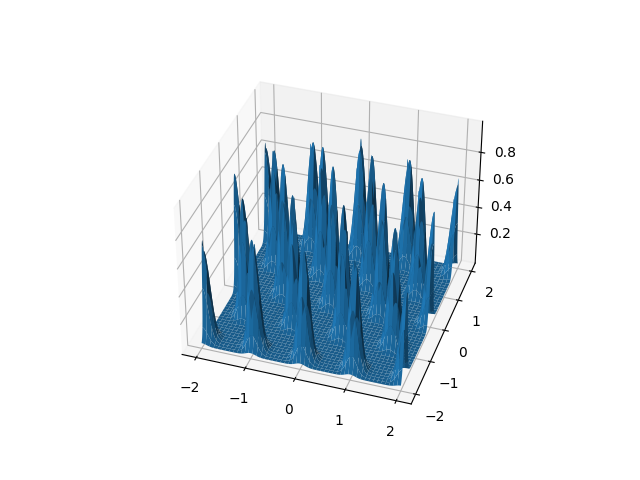
\includegraphics[width=90mm]{spikes.png}
\end{frame}

\begin{frame}
  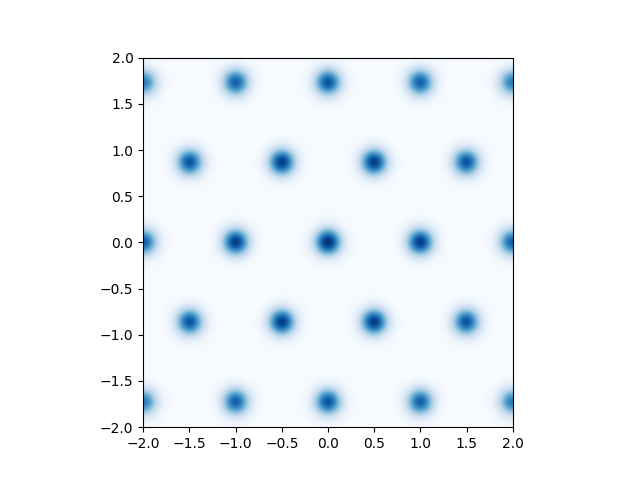
\includegraphics[width=90mm]{dots.png}
\end{frame}

\begin{frame}{The plan for the argument}
  Somehow, this is all supposed to come together to deliver a new proof of Frenkel's formula.
\end{frame}


\section{Section 5: Analytic problems and their solutions}

\begin{frame}
  \huge{Section 5: Analytic problems and their solutions}
\end{frame}

\begin{frame}{The problems we face}
  The main analytic difficulties we need to deal with are proving \emph{subelliptic estimates}
  \[
    \|u\|_{s+\varepsilon} \lesssim \|\Lc_bu\|_s+\|u\|_s,\quad \|v\|_{s+\varepsilon} \lesssim \|(\partial_t-\Lc_b)v\|_s+\|v\|_s
  \]
  where $\|\cdot\|_{s}$ is a scale of Sobolev spaces on $\gf\times G$ or $\gf\times G\times \Rl.$

  These are needed to prove that the exponential exists is at least trace-class, and also to establish the regularity of the kernel of $\exp(-t\Lc_b).$
\pause

  We also need some way to obtain estimates for
  \[
    |\exp(-tP_{b})((e,Y),(e,Y))|
  \]
  which exhibit the desired concentration on the co-roots. I will concentrate on this latter problem.
\end{frame}

\begin{frame}{The method of Gaffney and G\aa rding}
  I will illustrate the method we have with a very simple case: consider a diffusion operator
  \[
      K = \sum_{j} X_j^2
  \]
  where the $X_j$'s are antisymmetric vector fields satisfying the H\"ormander condition on some open set $U\subset \Rl^N.$
  \pause
  I will sketch out an argument that for $p,q\in U$ we have
  \[
        \exp(tK)(p,q) \lesssim \exp(-\frac{c}{t}\mathrm{dist}_{cc}(p,q)^2)
  \]
  where $\mathrm{dist}_{cc}$ is the Carnot-Caratheodory distance defined by $\{X_j\}.$
\end{frame}

\begin{frame}{Energy methods}
Let $u_0 \in L_2(U),$ and $u_t := \exp(tK)u_0.$ A simple computation yields the following:
\begin{lemma}
    Let $\phi \in C^\infty(U).$ We have
    \[
        \frac{d}{dt}\|\phi u_t\|^2 \leq 2\sum_j \|X_j(\phi)u_t\|^2.
    \]
\end{lemma}
Gaffney and G\aa rding's argument is to choose $\phi$ in an ingenious way.
\end{frame}

\begin{frame}{The ingenious choice of $\phi.$}
In particular, for $\phi = \exp(s\psi)$ where $s$ is a parameter to be chosen later, we have
\[
    \frac{d}{dt}\|\exp(s\psi)u_t\|^2 \leq 2s^2\|\exp(s\psi)u_t\|^2\left(\sum_{j}\|X_j(\psi)\|_{\infty}^2\right).
\]
By Gronwall's inequality, it follows that
\[
    \|\exp(s\psi)u_t\| \leq \|\exp(s\psi)u_0\|\exp(s^2t^2\sum_j \|X_j(\psi)\|_\infty^2).
\]
\end{frame}

\begin{frame}{The ingenious choice of $\phi.$}
Now select smooth functions $\nu$ and $\mu$ such that $u_0 = \nu u_0$, $\exp(s\psi)\nu = \nu$ and $\exp(s\psi)\mu = \exp(s)\mu.$
It follows that
\[
    \|\mu u_t\| = \exp(-s)\|\exp(s\psi)\mu u_t\| \leq \|\mu\|_\infty\exp(-s+s^2tk^2)\|\nu u_0\|.
\]
here,
\[
    k^2 = \sum_j \|X_j(\psi)\|_\infty^2.
\]
If we select $s = \frac{1}{2tk^2},$ this minimises $s^2tk^2-s$, and we get
\[
    \|\mu u_t\| \leq \exp(-\frac{1}{4t}k^{-2})\|u_0\|.
\]
\end{frame}

\begin{frame}
The infimum of $k$ is equivalent to one over the Carnot--Caratheodory distance between the supports of $\nu$ and $\mu.$ Hence,
\[
    \|\mu\exp(tK)\nu\|_{L_2\to L_2} \leq \exp(-\frac{d^2}{4t})\|\mu\|\|\nu\|.
\]
where $d$ is the Carnot--Caratheodory distance between the supports of $\nu$ and $\mu.$
\end{frame}

\begin{frame}{Complex interpolation}
From the $L_2$-estimate and an argument using Sobolev embedding and hypoellipticity, we arrive at
\[
    \exp(tK)(p,q) \lesssim \exp(-\frac{c}{t}\mathrm{dist}_{cc}(p,q)^2).
\]
\end{frame}

\begin{frame}{Kernel bounds with drift}
    Something much more interesting happens if we instead analyse an operator like
    \[
        K = \sum_{j} X_j^2 + Z
    \]
    where $Z$ is a new vector field. We can still do the argument, but we need to choose $\phi$ which moves along with the flow of $Z.$ This is how we arrive at the ``sub-Gaussian bounds with flow" needed for the concentration of the kernel of $\exp(-tP_b)$ on the co-roots.
\end{frame}

\section{Section 6: Conclusions}

\begin{frame}
  \Huge{Section 6: Conclusions}
\end{frame}

\begin{frame}{What next?}
  We have succeeded in proving Frenkel's formula by replacing some elementary representation theory and Poisson's summation formula by the most convoluted arguments imaginable. \\
  
  We can all agree that having new proofs of old results is worthwhile in itself, but...
  \textbf{What is the point of all this?}
  \begin{enumerate}
    \item{} Bismut's proof is \emph{totally different} to Frenkel's proof. Strikingly, \emph{no representation theory is needed}. We didn't even need the theorem of the highest weight. The coroot lattice turned up in the sum for completely geometric reasons.
    \item{} Bismut eventually extended his arguments to give totally new results, including his formulas for the heat kernel on symmetric spaces.
  \end{enumerate}
\end{frame}


\begin{frame}
\structure{\begin{center}
{\huge{}Thank you for listening!}\\
\begin{center}
{\Huge{}Happy Birthday Nigel!}
\end{center}
\par\end{center}}\end{frame}



\end{document}

